\section{Implementation}
In diesem Kapitel wird die Architektur des Gesamtsystems sowie die Hardware- und Software-Implementierung beschrieben.

\subsection{Architektur}
Das System besteht aus einer in C\# entwickelten Software, der Infrarotkamera Intel RealSense D455 und einem generischen Infrarotstift. Die Software ist plattformübergreifend kompatibel mit Windows, Linux und macOS.

\begin{figure}[H]
    \centering
    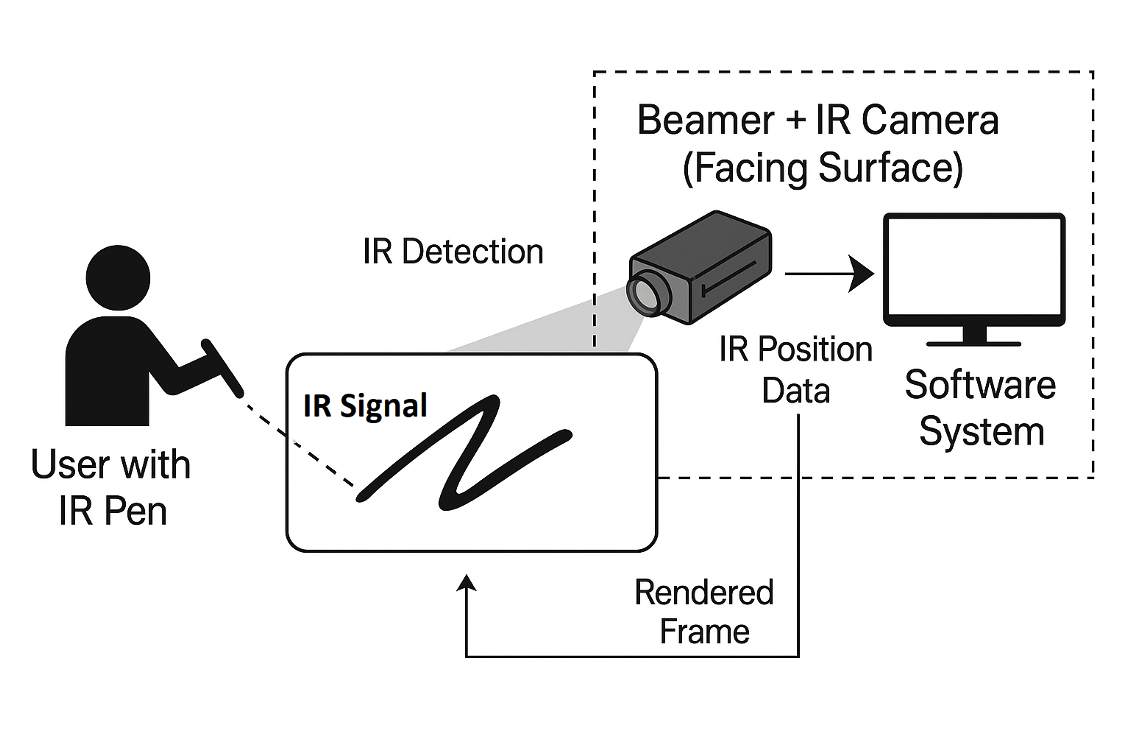
\includegraphics[width=0.5\linewidth]{graphics/system_uebersicht.png}
    \caption{Systemübericht}
    \label{fig:enter-label}
\end{figure}

\subsection{Setup}

Für das Setup muss die Kamera an den Computer angeschlossen und auf einen Bildschirm oder eine Projektionsfläche ausgerichtet werden. Anschliessend kann die Kalibrierung der Zeichenfläche über das Menü \texttt{Tools~→~Kalibrierung} (oben rechts in Abbildung \ref{fig:UI_screenshot}) gestartet werden. Im Kalibrierungsfenster muss der Infrarotstift nacheinander auf die fünf eingeblendeten Punkte gerichtet und aktiviert werden. Sobald sich das Fenster schliesst, ist das System bereit, um die Zeicheneingaben korrekt zu erfassen. Anschlissend können noch die PDF funktionen und die Gittergrösse angepasst werden.

\begin{figure}[H]
    \centering
    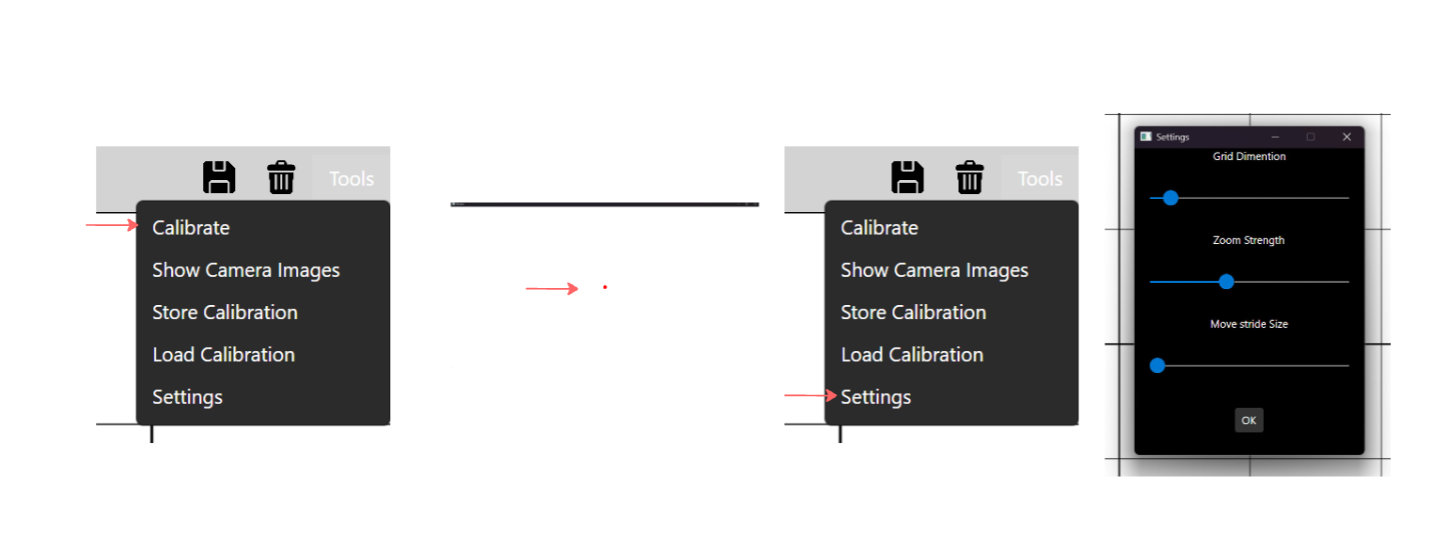
\includegraphics[width=0.8\linewidth]{graphics/anleitung_setup.png}
    \caption{Kurzanleitung für das Setup}
    \label{fig:anleitung_setup}
\end{figure}

Mit den Buttons Store- und Load Calibration kann die aktuelle Kalibration abgespeichert oder geladen werden um bei gleichem Setup die Einrichtung überspringen zu können.

\subsection{Hardware-Setup}
In diesem Abschnitt erläutern wir die eingesetzte Hardware sowie Anforderungen an mögliche Alternativen.

\vspace{0.5em}
\subsubsection{Infrarotstift}
Wir verwenden einen generischen Infrarotstift (siehe Anhang für Verkaufslink \ref{hw-info}). Dieser verfügt über eine Infrarot-LED, die durch das Eindrücken der Spitze oder das Drücken einer Taste auf der Oberseite aktiviert wird.

\begin{figure}[H]
    \centering
    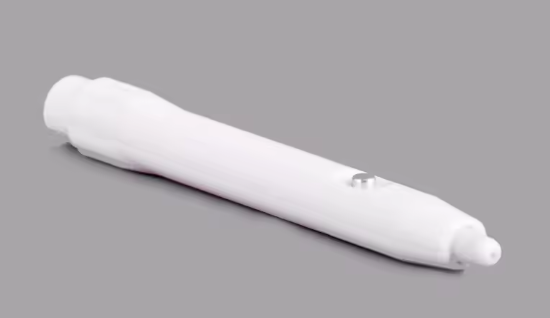
\includegraphics[width=0.5\linewidth]{bild_pen.png}
    \caption{Bild eienes Infrarotstiftes}
    \label{fig:enter-label}
\end{figure}

Es kann auch ein beliebiger anderer Infrarotstift verwendet werden. In der nachfolgenden Abbildung ist ein einfaches elektrisches Schema für die Mindestanforderung an die Hardware.

\begin{figure}[H]
    \centering
    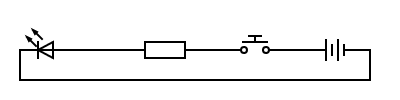
\includegraphics[width=0.5\linewidth]{schema_pen.png}
    \caption{Beispiel Schema für Infrarotstift}
    \label{fig:enter-label}
\end{figure}


\clearpage
%\vspace{0.5em}
\subsubsection{Infrarotkamera}

Wir verwenden die Infrarotkamera Intel RealSense D455, da sie dem SCDH bereits zur Verfügung stand. Die D455 verfügt über zwei Infrarotkameras, eine RGB-Kamera sowie einen steuerbaren Infrarot-Laser. Für unsere Anwendung genügt eine der beiden IR-Kameras.

\begin{figure}[H]
    \centering
    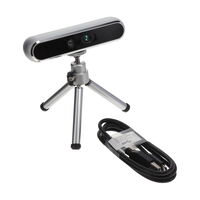
\includegraphics[width=0.5\linewidth]{graphics/bild_d455.jpg}
    \caption{Intel RealSense D455}
    \label{fig:enter-label}
\end{figure}

Zur Verbesserung der Bildqualität unter schwierigen Lichtverhältnissen wurde eine Filterfolie angebracht (Dämpfungskurve ersichtlich in Abbildung\ref{fig:filter_kurve}). Als Ersatz eignen sich prinzipiell alle Intel RealSense IR-Kameras mit SDK-Unterstützung. Mit Anpassungen in der InfraredCamera-Klasse können auch andere Kameramodelle eingesetzt werden.

\clearpage

\subsection{Software}
In diesem Abschnitt stellen wir zentrale Softwarekomponenten vor.

\vspace{0.5em}
\subsubsection{Benutzeroberfläche (UI)}
\begin{figure}[H]
    \centering
    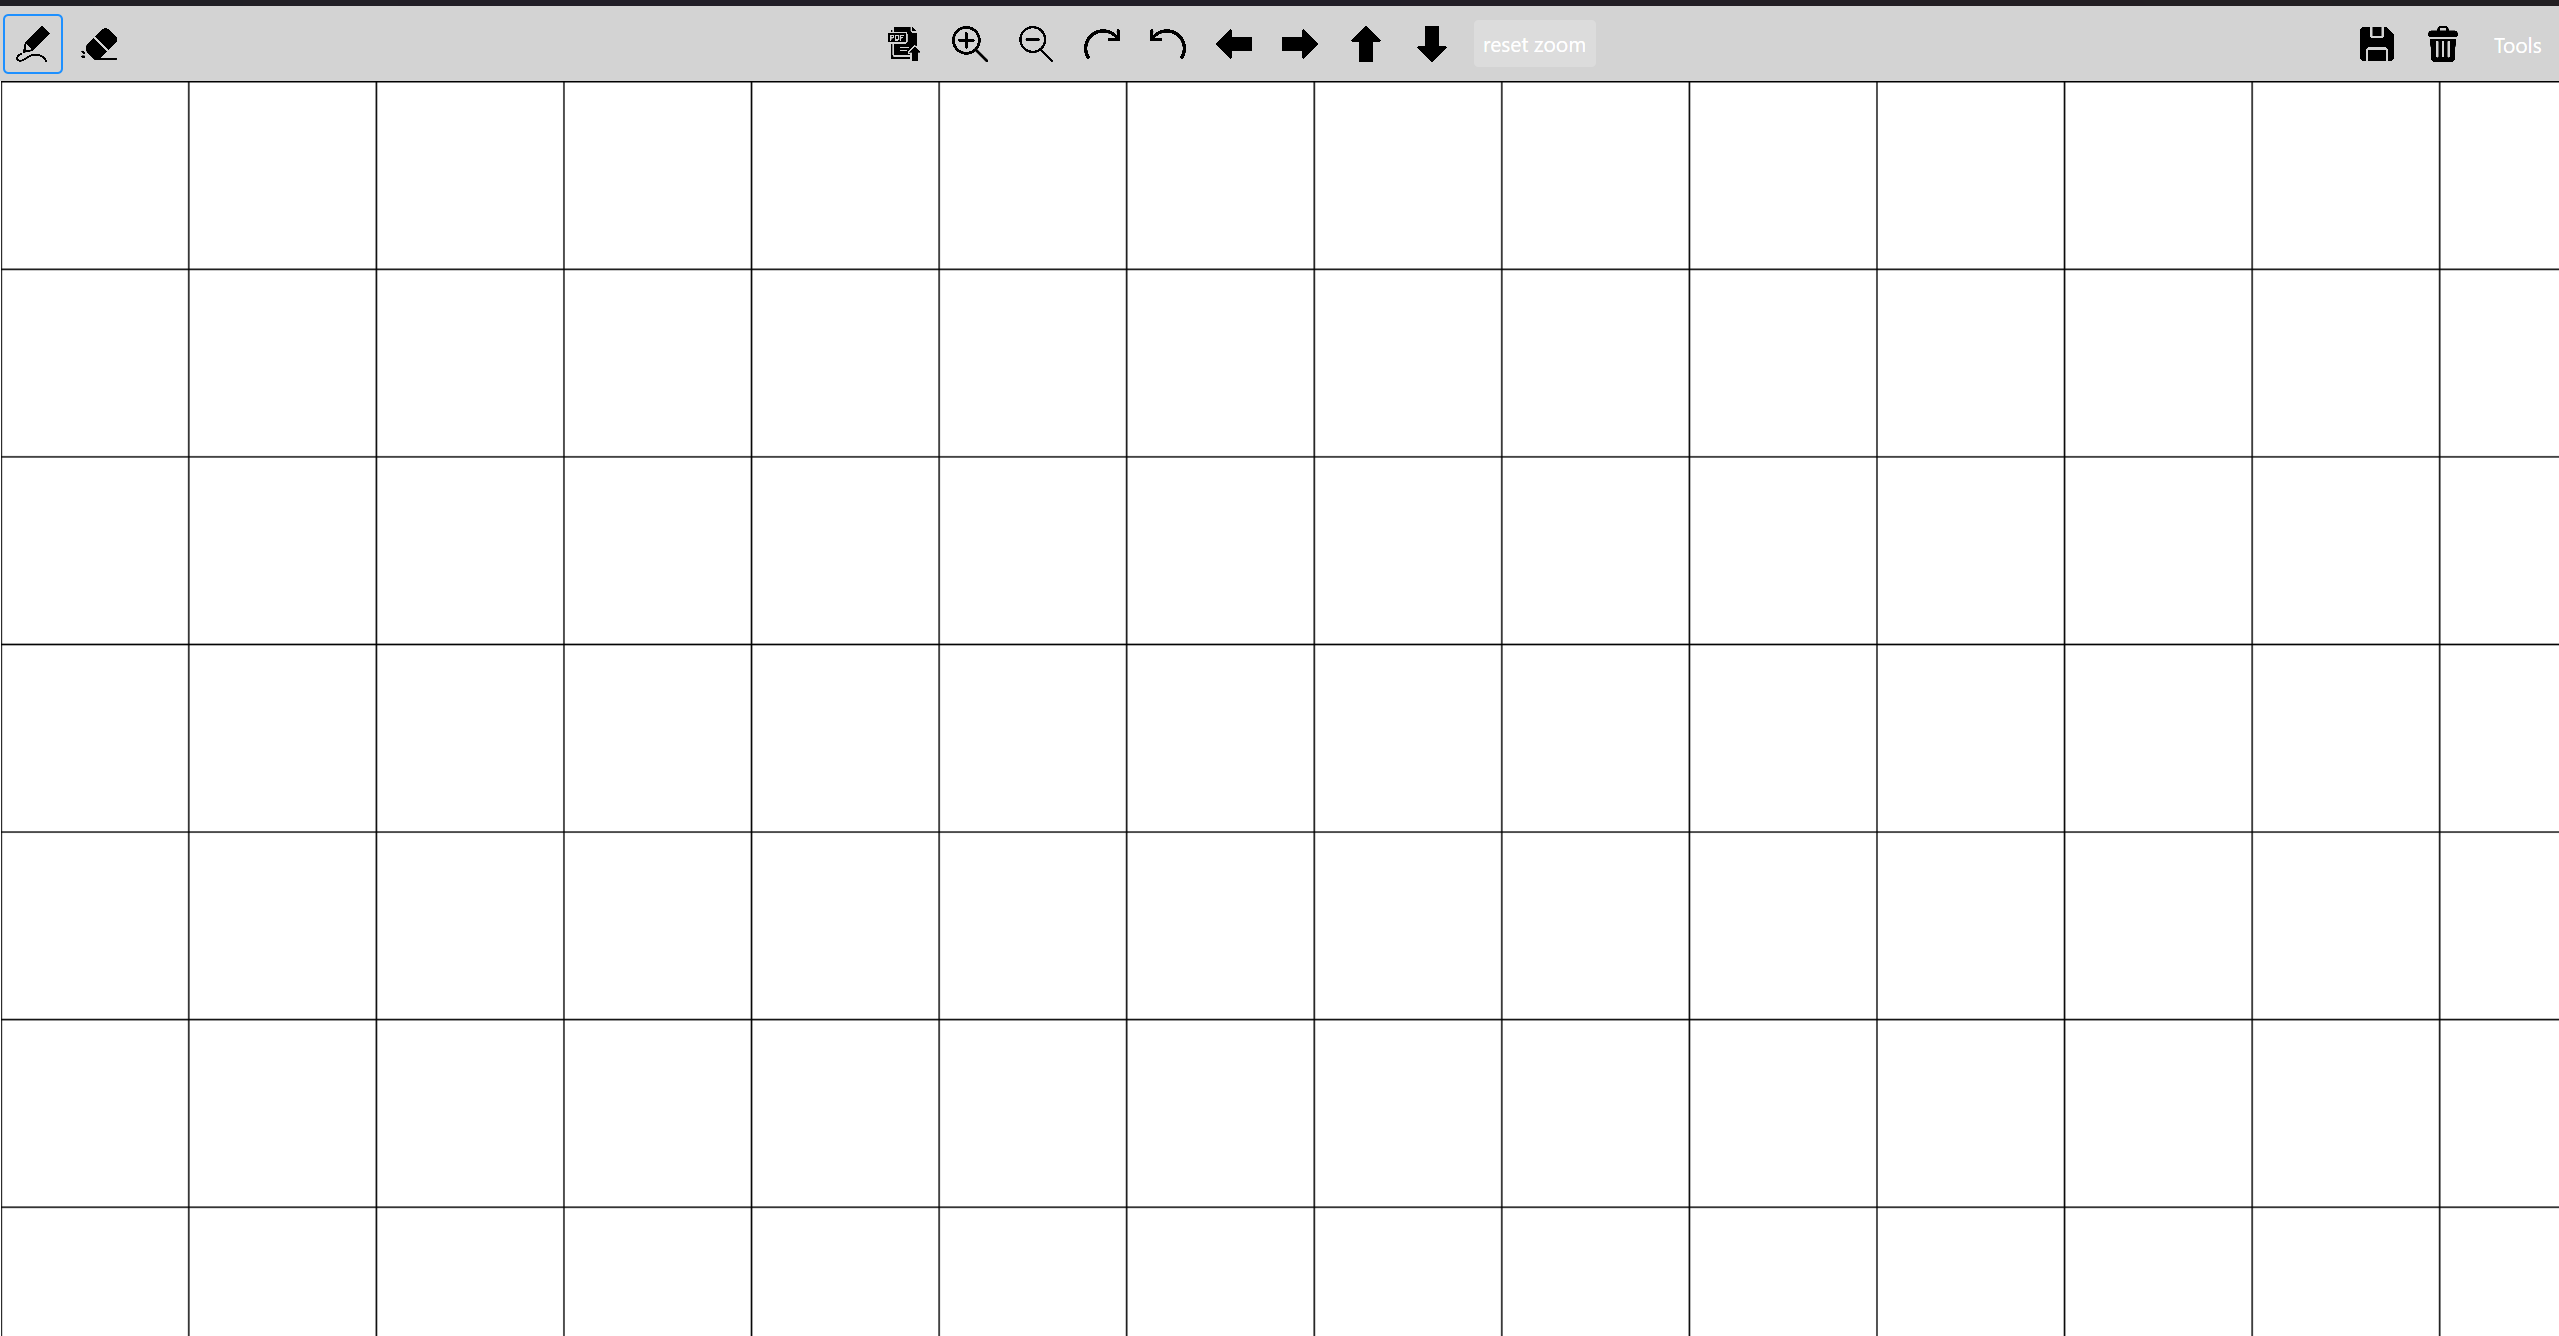
\includegraphics[width=0.75\linewidth]{graphics/ui_screenshot.png}
    \caption{UI Screenshot}
    \label{fig:UI_screenshot}
\end{figure}

Die Benutzeroberfläche besteht aus der Zeichenfläche und einer Werkzeugleiste.\\
Die Werkzeugleiste stellt Funktionen wie Farbauswahl, PDF-Import, Zoom und Pan bereit (detaillierte Dokumentation im Anhang). Für die UI wurde hauptsächlich die Avalonia-Library verwendet.

\vspace{0.5em}
\subsubsection{Zeichenfläche}

Die Zeichenfläche basiert auf einer SKWritableBitmap in einem SKCanvas aus der SkiaSharp-Library. Zeicheneingaben mit Maus oder IR-Stift werden über diese Bitmap dargestellt.

\begin{figure}[H]
  \begin{minipage}{0.48\textwidth}
    \centering
    \frame{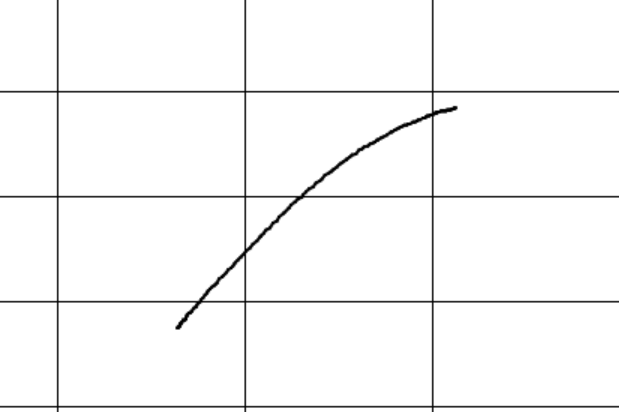
\includegraphics[width=0.9\linewidth]{graphics/bild_strich_in_zeichnungsflaeche.png}}
    \caption{Zeichnungsstrich}
    \label{Fig:Data1}
  \end{minipage}
  \hfill
  \begin{minipage}{0.48\textwidth}
    \centering
    \frame{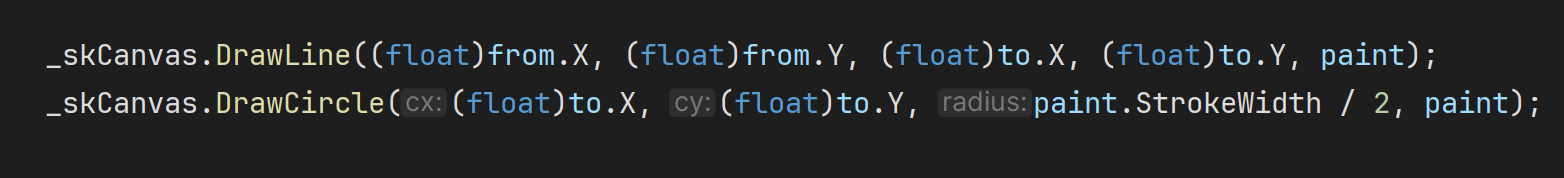
\includegraphics[width=0.9\linewidth]{graphics/code_drawline.png}}
    \caption{Code zur Darstellung eines Striches}
    \label{Fig:Data2}
  \end{minipage}
\end{figure}

\clearpage

Für die Verarbeitung der Stift-Eingaben ist ein Eventhandler zuständig, der auf ein CameraEvent der Klasse InfraredCamera reagiert. Dieser Event informiert die UI-Klasse über erkannte Punkte. Für alle erkannten Punkte in der Liste wird folgende Verarbeitungspipeline durchlaufen:

\begin{figure}[H]
    \centering
    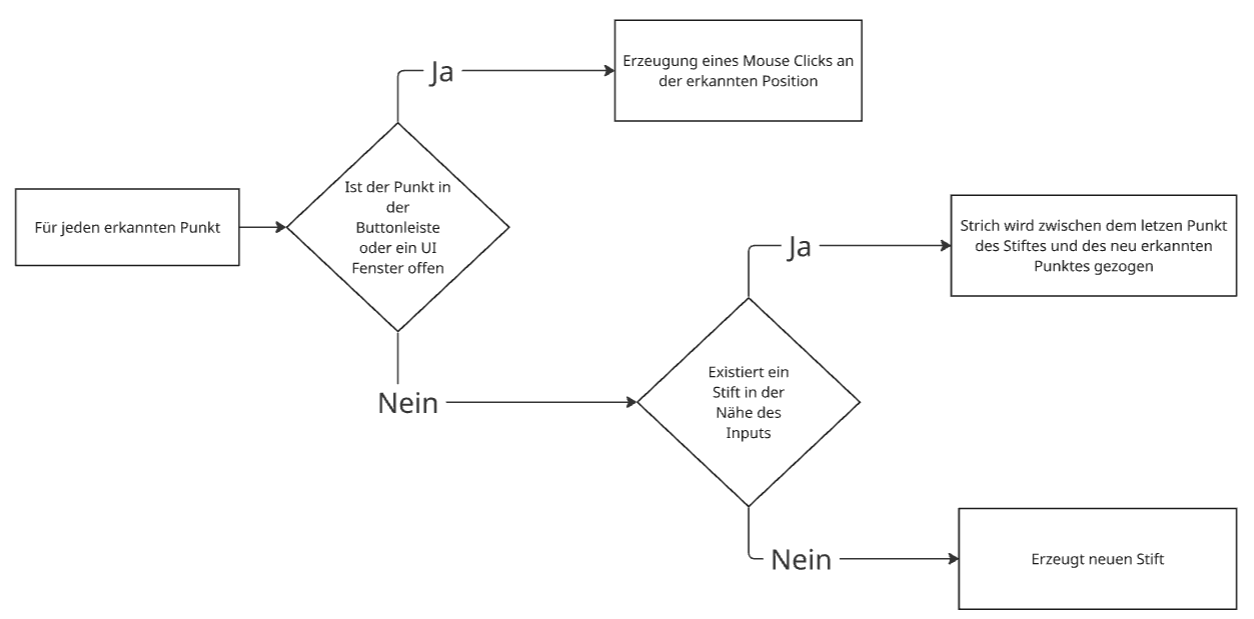
\includegraphics[width=\linewidth]{schema_ablauf_punktdetektion_uiklasse.png}
    \caption{Ablaufschema für die Verarbeitung der erkannten Punkte}
    \label{fig:enter-label}
\end{figure}

Zuerst wird geprüft, ob sich der Punkt im Bereich der Werkzeugleiste befindet. Ist dies der Fall, oder ist durch die Leiste ein Fenster geöffnet, wird der Punkt in einen Mausklick im entsprechenden Screen-Space umgewandelt. So können plattformunabhängig auch systemeigene Dialoge wie etwa Dateiauswahlen bedient werden.
Handelt es sich nicht um einen Steuerungsinput, wird der Punkt als Zeichenbefehl interpretiert. Zur Darstellung einer Linie werden jeweils der aktuelle sowie der letzte Punkt eines Stifts benötigt. Das Tracking erfolgt über eine Liste aller aktiven Stifte, wobei für jeden der letzte Punkt und ein Zeitstempel gespeichert werden. Neue Punkte werden dem wahrscheinlichsten existierenden Stift zugeordnet, basierend auf Distanz und Zeitdifferenz. Falls eine Zuordnung erfolgt, wird eine Linie gezeichnet und die Stiftinformationen aktualisiert.

\clearpage
%\vspace{0.5em}
\subsubsection{Infrarot Stift Erkennung}

Die Erkennung der Stiftspitze erfolgt vollständig innerhalb der InfraredCamera-Klasse. Die Kamera wird über die Intel RealSense SDK angesteuert, die Erkennung erfolgt mit OpenCV.

\begin{figure}[H]
    \centering
    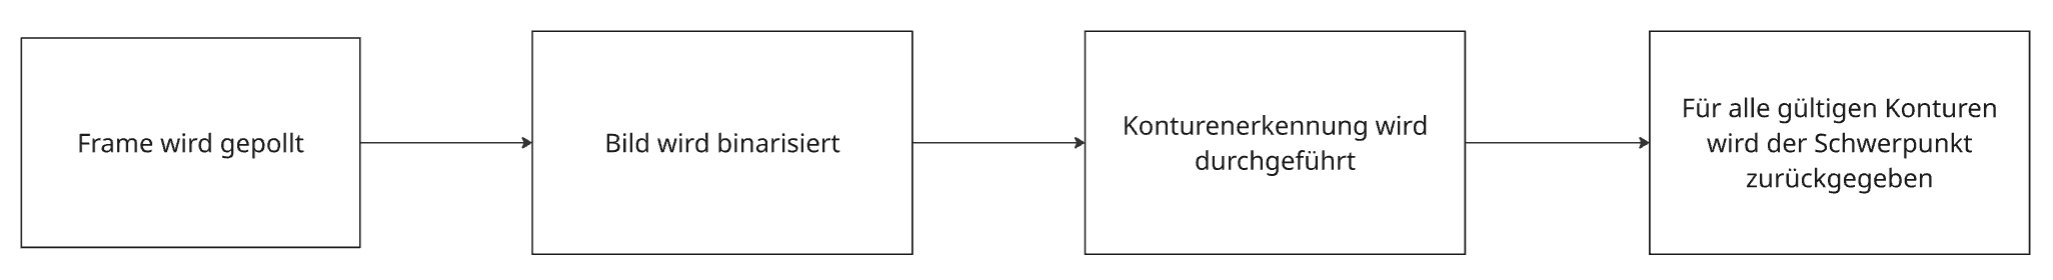
\includegraphics[width=\linewidth]{schema_pen_dedection.png}
    \caption{Ablaufsschema der Stift erkennung}
    \label{fig:enter-label}
\end{figure}

Zunächst werden Bilder der IR-Kamera gepollt:

\begin{figure}[H]
    \begin{minipage}{0.48\textwidth}
    \centering
    \frame{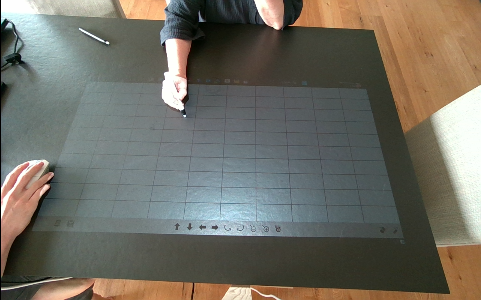
\includegraphics[width=0.9\linewidth]{rgb.png}}
    \caption{Sicht der RGB Kamera}
    \label{Fig:Data1}
  \end{minipage}
  \hfill
  \begin{minipage}{0.48\textwidth}
    \centering
    \frame{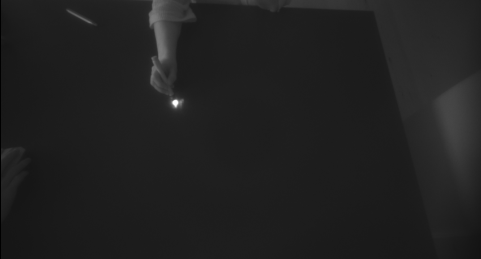
\includegraphics[width=\linewidth]{ir.png}}
    \caption{Sicht der IR Kamera}
    \label{Fig:Data2}
  \end{minipage}
\end{figure}

Diese Bilder werden mittels einfacher Threshold-Binarisierung segmentiert:

\begin{figure}[H]
    \begin{minipage}{0.48\textwidth}
    \centering
    \frame{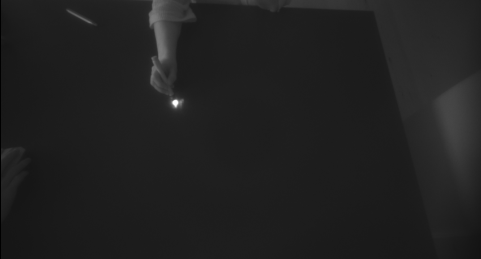
\includegraphics[width=0.9\linewidth]{ir.png}}
    \caption{Sicht der IR Kamera}
    \label{Fig:Data1}
  \end{minipage}
  \hfill
  \begin{minipage}{0.48\textwidth}
    \centering
    \frame{
\includegraphics[width=0.9\linewidth]{graphics/binarisiert.png}}
    \caption{Segmentiertes Bild}
    \label{Fig:binarisiert}
  \end{minipage}
\end{figure}

In den segmentierten Bildern werden mit OpenCV die Konturen erkannt. Der Schwerpunkt jedes Blobs in dem segmentierten Bild (Abbildung \ref{Fig:binarisiert}) wird über das zentrale Moment berechnet und als Stiftspitze interpretiert.

\[
x = \frac{M_{10}}{M_{00}}, \quad y = \frac{M_{01}}{M_{00}}
\]
\clearpage

Der erkannte Bildpunkt wird anschliessend per Homographie in den Screenspace übersetzt und zur Liste der gültigen Eingabepunkte hinzugefügt. Die Homographie-Matrix wird ebenfalls mit OpenCV berechnet:

\begin{figure}[H]
    \centering
    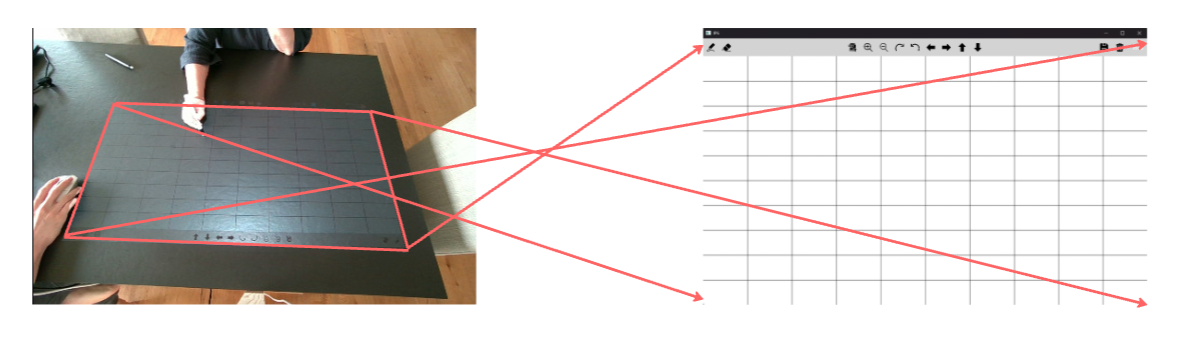
\includegraphics[width=0.9\linewidth]{graphics/homography_graphic.png}
    \caption{Verbildlichung der Homography}
    \label{fig:enter-label}
\end{figure}

\vspace{0.5em}
\subsubsection{Kalibration}

Für die Kalibration werden nacheinander fünf Punkte auf der Zeichenfläche angezeigt:

\begin{figure}[H]
    \centering
    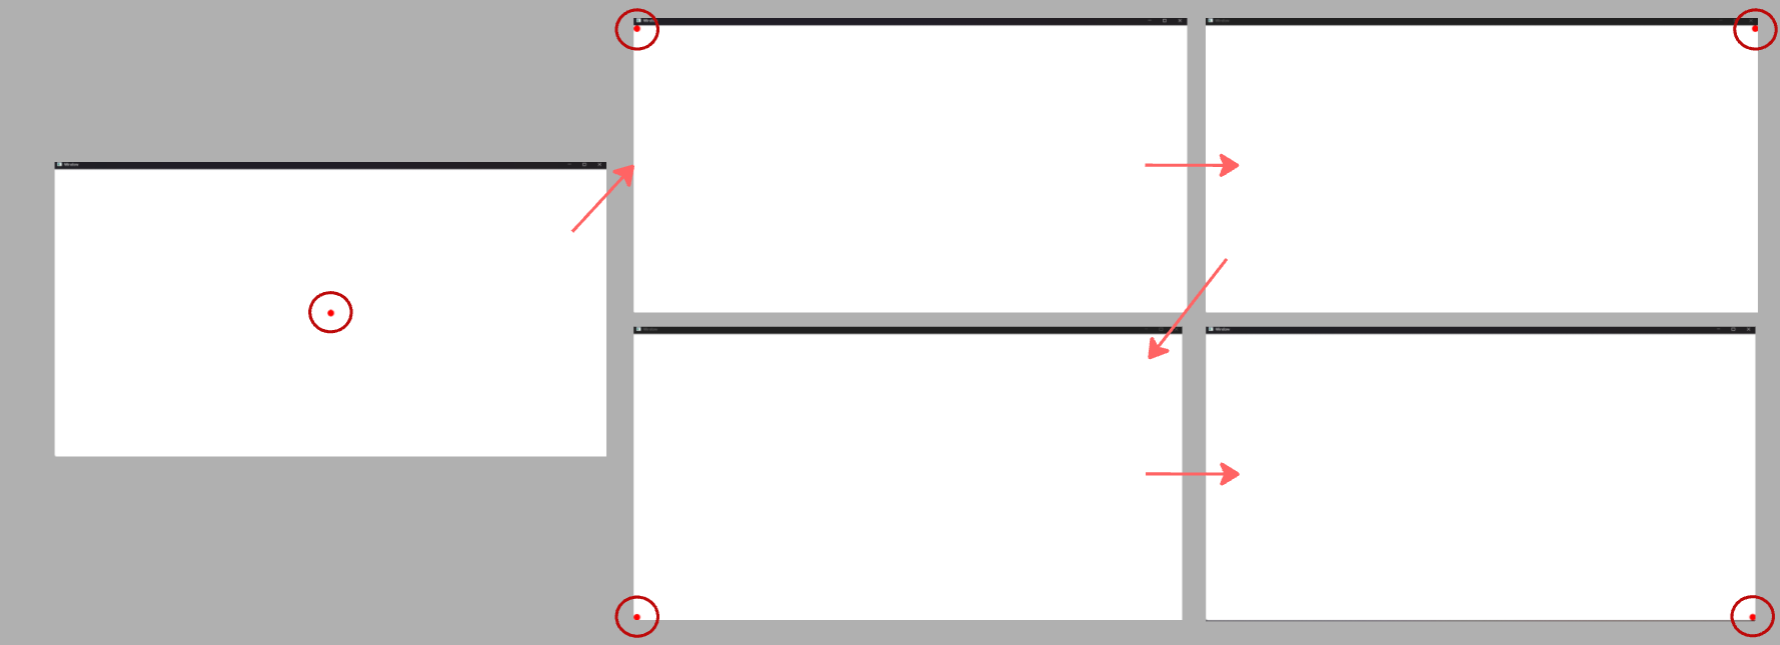
\includegraphics[width=0.9\linewidth]{graphics/ablauf_kalibration.png}
    \caption{Kalibrationsablauf}
    \label{fig:placeholder}
\end{figure}

Bei jedem dieser Punkte wird auf ein CameraEvent gewartet. Der jeweils zuerst erkannte Punkt im Kamerabild wird als entsprechender Kalibrationspunkt im Kameraraum gespeichert.

Diese Punkte im Kamerakoordinatensystem werden anschliessend zusammen mit den bekannten Referenzpunkten im Screen-Space an OpenCV übergeben, um die Homographie-Matrix zu berechnen. Nach erfolgreicher Berechnung der Homographie-Matrix ist die Kalibration abgeschlossen und das Kalibrationsfenster wird automatisch geschlossen.

